\documentclass[extra]{gji}
%~ \documentclass[extra, referee]{gji}

\usepackage[utf8]{inputenc}
\usepackage{timet}
\usepackage{amsmath}
\usepackage{graphicx}
\usepackage{todonotes} % to make annotations on margins
%~ \usepackage[disable]{todonotes} % to disable annotations on margins

\usepackage{url}
\usepackage[pdftex,colorlinks=true]{hyperref}
\hypersetup{
    allcolors=blue,
}


\begin{document}

\title[Variable Density Tesseroids]{
    Gravitational field calculation in spherical coordinates using variable
    densities in depth
}
\author[S.R. Soler, A. Pesce, L. Uieda and M.E. Gimenez]{
    Santiado R. Soler$^{1,2}$, Agustina Pesce$^{1,2}$, Leonardo Uieda$^3$ and
    Mario E. Gimenez$^{1,2}$ \\
    $^1$CONICET, Argentina. e-mail: santiago.r.soler@gmail.com\\
    $^2$Instituto Geofísico Sismológico Volponi, Universidad Nacional de
    San Juan, Argentina\\
    $^3$Department of Earth Sciences, SOEST, University of Hawai‘i at
    M\={a}noa, Honolulu, Hawaii, USA
}


\maketitle

\begin{summary}
We present a new methodology to compute the gravitational fields generated by
any tesseroid whose density varies continuously in depth, i.e. a forward
gravity model in spherical coordinates for varying densities on the radial
direction.
It numerical approximates these gravitational fields through the
Gauss-Legendre Quadrature along with two discretization algorithms that
increase its accuracy by subdividing the tesseroid into smaller ones.
The first one is a preexisting adaptive discretization algorithm that reduces
the errors due to the distance between the tesseroid and the computation
point.
While the second one  is a new density-based discretization algorithm that
decreases the errors introduced by the variation of the density function.
The amount of discretizations made by each algorithm is indirectly controlled
by two predefined scalar values: the distance-size ratio $D$ for the former
and the delta ratio $\delta$ for the latter.
We have also obtained analytical solutions for a spherical shell with variable
density and compared them with the results of the numerical model in case of a
linear and an exponential density function.
These comparisons allowed to obtain default values for the distance-size and
the delta ratio in order to guarantee the accuracy of the forward model.
The resulting optimal values of $D$ for the gravity potential, the components
of its gradient and the Marussi tensor components are 1, 2 and 8,
respectively.
While a $\delta=0.2$ is needed for the computation of the gravitational
potential and its gradient components and a $\delta=0.01$ must be used for
the Marussi tensor components.
We have finally tested this new methodology by modelling the Neuqu\'en
sedimentary basin, located to the east of the Andes between 32$^\circ$S and
40$^\circ$S latitude, assigning an exponential density variation to it and
computing all the gravitational fields it generates.
\end{summary}

\begin{keywords}
Numerical modelling, Numerical approximations and analysis, Gravity anomalies
and Earth structure, Satellite gravity
\end{keywords}


\section{Introduction}

The lithosphere's density variation with depth has been studied for close to a
century.
Over this time period,
several density-depth relations have been proposed for different rock types
\citep[e.g.,][]{Maxant1980, Rao1986, Rao1993, Rao1994}.
Furthermore, depth-variable densities have been used in forward and
inverse gravity modeling, mostly applied to sedimentary basins
\citep{Cordell1973, Rao1986, Cowie1990, Rao1993, Rao1994, Zhang2001,
Welford2010}.
These forward gravity models have been developed for two or three dimensional
bodies in Cartesian coordinates, which limits the applications to local scales.
The advent of satellite gravimetry has provided gravity field
measurements with global coverage, enabling modelling and interpretation on regional and
global scales.
Hence, designing forward modeling methods that reproduce the gravity anomalies for
such scales is of high importance.

To take into account the curvature of the Earth, many global forward modeling methods
are defined in geocentric spherical coordinates.
A common approach is to discretize the Earth into tesseroids (spherical prisms),
which are defined by pairs of latitude, longitude, and
radial boundaries (see Fig.~\ref{fig:tesseroid}).
The gravitational fields generated by an arbitrary
tesseroid on any external point are given by volume
integrals that are generally approximated by numerically.
The literature offers two main approaches: one involves Taylor series expansion
\citep{Heck2007, Grombein2013} while the other makes use of Gauss-Legendre
Quadrature (GLQ)
\citep{Asgharzadeh2007, Wild-Pfeiffer2008, Li2011, Uieda2016}.
The Taylor series expansion is not well suited to develop an algorithm for
a density varying with depth according to an arbitrary function.
Different series expansion terms would have to obtained for each density function
desired.
Conversely, an arbitrary density function can be included in the GLQ without
any change to the integration method.

\begin{figure}
\centering
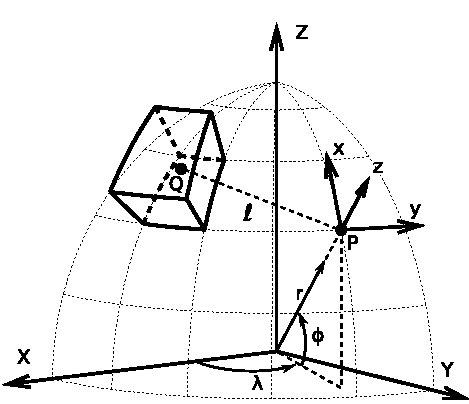
\includegraphics[width=0.9\linewidth]{figures/tesseroid-uieda.pdf}
\caption{
    A tesseroid (spherical prism) in a geocentric spherical coordinate system, with a
    computation point $P$ and its local north oriented Cartesian coordinate system.
    After \citet{Uieda2015}.
}
\label{fig:tesseroid}
\end{figure}

The main challenge of the GLQ integration is loss of accuracy when the computation point
gets closer to the tesseroid \citep{Ku1977}.
\citet{Uieda2016} built on the adaptive discretization algorithm of \citet{Li2011}
to automatically obtain integration results with 0.1\% accuracy.
The algorithm consist in recursively splitting the tesseroid into smaller ones when a
threshold is exceeded,
namely when the normalized distance to the computation point is greater than a
``distance-size ratio'' ($D$).
\citet{Uieda2016} have also obtained standard values of $D$
for the gravitational potential, acceleration, and gradient tensor components
by comparing the numerical model with the fields generated by a spherical shell.

We present a new algorithm for computing the gravitational fields generated by any
tesseroid with an arbitrary continuous density function on any external point.
It is based on the GLQ approximation and the adaptive discretization of
\citet{Uieda2016}, which we extend to include a new density-based discretization step.
In order to ensure the accuracy of the numerical approximation we have
determined optimal values for the controlling parameters by
comparing the numerical approximation with analytical solutions for
spherical shells.
Finally, we applied the methodology to model the Nequen basin, Argentina, using
tesseroids with an exponentially increasing density with depth.


%%%%%%%%%%%%%%%%%%%%%%%%%%%%%%%%%%%%%%%%%%%%%%%%%%%%%%%%%%%%%%%%%%%%%%%%%%%%%%

\section{Methodology}

We define an external computation point $P(r, \phi, \lambda)$ in a geocentric spherical
coordinate system at a radius $r$, geocentric latitude $\phi$, and longitude $\lambda$
where the gravitational fields are going to be calculated.
The first and second derivatives of the gravitational potential are taken with
respect to the local north-oriented Cartesian coordinate system of $P$
(Fig.~\ref{fig:tesseroid}).
\citet{Grombein2013} provide efficient formulations for the volume integrals of the
gravitational potential and its first and second derivatives of a tesseroid with
homogeneous density.
Here, we will assume that the tesseroid has a density varying with $r$ according to an
arbitrary function $\rho(r)$.
Thus, the integrals for the gravitational fields are slightly modified to

\begin{equation}
    V(r,\phi,\lambda) = G
    \int\limits_{\lambda_1}^{\lambda_2}
    \int\limits_{\phi_1}^{\phi_2}
    \int\limits_{r_1}^{r_2}
    \frac{\rho(r')}{\ell} \kappa \,  dr' d\phi' d\lambda',
\label{eq:tesseroid-pot}
\end{equation}

\begin{equation}
    g_{\alpha}(r,\phi,\lambda) = G
    \int\limits_{\lambda_1}^{\lambda_2}
    \int\limits_{\phi_1}^{\phi_2}
    \int\limits_{r_1}^{r_2}
    \rho(r') \frac{\Delta_\alpha}{\ell^3}
    \kappa \, dr' d\phi' d\lambda',
\label{eq:tesseroid-grav}
\end{equation}

\noindent and

\begin{equation}
    g_{\alpha\beta}(r,\phi,\lambda) = G
    \int\limits_{\lambda_1}^{\lambda_2}
    \int\limits_{\phi_1}^{\phi_2}
    \int\limits_{r_1}^{r_2}
    \rho(r') I_{\alpha\beta} \, \kappa \, dr' d\phi' d\lambda' ,
    \label{eq:tesseroid-tensor}
\end{equation}

\noindent in which

\begin{equation}
    I_{\alpha\beta} =
    \left(
        \frac{3\Delta_{\alpha} \Delta_{\beta}}{\ell^5} -
        \frac{\delta_{\alpha\beta}}{\ell^3}
    \right) ,
    \label{eq:tesseroid-tensor-kernel}
\end{equation}

\noindent $\alpha, \beta \in \{x, y, z\}$, $\delta_{\alpha\beta}$ is Kronecker's delta,
$G = 6.674\times10^{-11}\, \text{m$^3$kg$^{-1}$s$^{-1}$}$ is the gravitational constant
and

\begin{equation}
    \Delta_x = r'[\cos\phi\sin\phi' - \sin\phi\cos\phi'
               \cos(\lambda' - \lambda)],
\end{equation}
\begin{equation}
    \Delta_y = r' \cos \phi' \sin(\lambda' - \lambda),
\end{equation}
\begin{equation}
    \Delta_z = r' \cos \psi - r,
\end{equation}
\begin{equation}
    \kappa = {r'}^2 \cos \phi',
\end{equation}
\begin{equation}
    \ell = \sqrt{{r'}^2 + r^2 - 2 r r' \cos \psi},
\label{eq:ell}
\end{equation}
\begin{equation}
    \cos\psi = \sin\phi\sin\phi' + \cos\phi\cos\phi'
                 \cos(\lambda' - \lambda).
\label{eq:cospsi}
\end{equation}

\subsection{Gauss-Legendre Quadrature integration}

Applying a $N$th order GLQ, we can approximate each integral in equations
\ref{eq:tesseroid-pot}, \ref{eq:tesseroid-grav} and \ref{eq:tesseroid-tensor} by a
weighted sum of the integration kernel evaluated on the roots of an $N$th order Legendre
polynomial \citep[p.~390]{Hildebrand1987}.
Unlike the homogeneous density case, the radial density function $\rho(r)$ must also be
included in the integration and evaluated on the Legendre polynomial roots (i.e.,
quadrature nodes).

\iftwocol{
\begin{equation}
    \begin{split}
        \iiint\limits_\Omega \rho(r') g(r', \phi', \lambda')
        d\Omega \approx& \\
        A
        \sum\limits_{i=1}^{N^r}
        \sum\limits_{j=1}^{N^\phi}
        \sum\limits_{k=1}^{N^\lambda}
        & W_i^r W_j^\phi W_k^\lambda \rho(r_i) g(r_i, \phi_j, \lambda_k),
    \end{split}
\label{eq:glq-var-dens}
\end{equation}
}{
\begin{equation}
    \iiint\limits_\Omega \rho(r') g(r', \phi', \lambda') d\Omega \approx
    A
    \sum\limits_{i=1}^{N^r}
    \sum\limits_{j=1}^{N^\phi}
    \sum\limits_{k=1}^{N^\lambda}
    W_i^r W_j^\phi W_k^\lambda \rho(r_i) g(r_i, \phi_j, \lambda_k),
\label{eq:glq-var-dens}
\end{equation}
}

\noindent where

\begin{equation}
    A =
    \frac{(\lambda_2 - \lambda_1)(\phi_2 - \phi_1)(r_2 - r_1)}{8},
\end{equation}

\noindent $(r_i, \phi_j, \lambda_k)$ are the quadrature nodes, and $W_i^r$ are the
quadrature weights.


\subsection{Adaptive Discretization}

\citet{Ku1977} noticed that the GLQ integration
becomes less accurate when the computation point is closer to the
mass element.
One way to prevent this from happening would be to increase the GLQ order.
Doing so would uniformly increase the number of point masses inside the
tesseroid volume.
However, an increase in the point mass concentration is only required close to the
computation point \citep{Uieda2016}.
Alternatively, \citet{Li2011} proposed an adaptive
discretization algorithm which keeps the GLQ order fixed and divides the
tesseroid based on a ratio between the distance to the computation
point and its dimensions.
This algorithm produces a more efficient computation because an increased concentration
of point masses is produced where it is needed more.
\citet{Uieda2016} developed a modified version of this algorithm, which we will use
here.
What follows is a summary of the algorithm and the reader is referred to
\citet{Uieda2016} for a detailed description.

The following algorithm computes the gravitational fields at a given point at $(r, \phi,
\lambda)$ due to a tesseroid with its geometric center at $(r_t, \phi_t, \lambda_t)$ and
dimensions $L_r$, $L_\phi$, and $L_\lambda$ given by

\begin{equation}
    L_\lambda = r_2 \arccos(\sin^2\phi_t +
        \cos^2\phi_t\cos(\lambda_2 - \lambda_1)),
    \label{eq:sizelon}
\end{equation}

\begin{equation}
    L_\phi = r_2 \arccos(\sin\phi_2\sin\phi_1 + \cos\phi_2\cos\phi_1),
\end{equation}

and

\begin{equation}
    L_r = r_2 - r_1.
    \label{eq:sizer}
\end{equation}

\textit{Step 1}: Check that the tesseroid satisfies the following inequality for each
dimension $L_i$ of the tesseroid:

\begin{equation}
    \frac{d}{L_i} \geq D,
    \label{eq:condition}
\end{equation}

\noindent
in which $D$ is a positive scalar called the distance-size ratio and $d$ is the distance
between the computation point and the geometric center of the tesseroid

\begin{equation}
    d = \left[
        r^2 + r_t^2 - 2 r r_t \cos\psi_t
        \right]^{\frac{1}{2}} ,
    \label{eq:distance}
\end{equation}

\begin{equation}
    \cos\psi_t =
        \sin\phi\sin\phi_t + \cos\phi\cos\phi_t\cos(\lambda - \lambda_t) .
\end{equation}

\textit{Step 2}:
If none of the dimensions of the tesseroid fail inequality
\ref{eq:condition}, then compute the gravitational effect of the tesseroid using a
second-order GLQ (Eq. \ref{eq:glq-var-dens}).
Add the computed effect to a running total.

\textit{Step 3}:
If any dimension fails inequality \ref{eq:condition}, split the tesseroid in half along
the offending dimensions.
Repeat steps 1-3 for all smaller tesseroids until none are left.

\textit{Final step}:
By the end of the algorithm, the running total will be the gravitational effect of the
tesseroid.

Notice that the distance-size ratio $D$ determines how many
times the tesseroids will be divided.
Therefore, it effectively regulates both the accuracy of the algorithm and its
computation time.
An optimal value for $D$ cannot be directly calculated from the desired accuracy level.
Instead, it is empirically determined by comparing the numerical results with the
analytical solution for a spherical shell.
\citet{Uieda2016} used a shell with homogeneous density to determine optimal values of
$D$.
Here, we will repeat the numerical experiment using analytical expressions for shells
with density varying according to exponential and linear functions of $r$.


\subsection{Density-based Discretization Algorithm}

The numerical integration of an arbitrary density function introduces
a new type of problem:
the integration error from using only a few nodes to discretize the density function.
The adaptive discretization may help
to reduce this kind of error.
However, it does not take into account the density function
and hence it is not well suited to fully perform this task.

We have developed a complementary discretization
algorithm that takes into account the variations of the density function.
This density-based discretization happens prior to the adaptive discretization described
in the previous section.
In short, the algorithm divides the tesseroid along the radial dimension at the
depths at which the \emph{maximum density variations} take place.

Consider an \emph{original} tesseroid with density given by the function $\rho(r')$.
Before the density-based discretization starts,
we normalise the density function to the range $[0, 1]$ as follows

\begin{equation}
    \rho_n(r') =
    \frac{\rho(r') - \rho_\text{min}}{\rho_\text{max} - \rho_\text{min}},
\end{equation}

\noindent in which $\rho_\text{min}$ and $\rho_\text{max}$ are the minimum and maximum
density values inside the tesseroid boundaries.
We emphasize that this normalised density function will not be modified throughout the
algorithm.
In case the density function is constant, both maximum and minimum densities will be
equal and the density-based discretization algorithm will not be applied.

The algorithm is comprised of the following steps
(Fig. \ref{fig:density-discretization-algorithm}):

\textit{Step 1}:
Define a linear function $\rho_l(r')$ that assumes
the same values as the normalised density $\rho_n(r')$ at the boundaries of the
tesseroid ($r_1$ and $r_2$):

\begin{equation}
    \rho_l(r') =
    \frac{ \rho_n(r_2) - \rho_n(r_1) }{ r_2 - r_1 } (r' - r_1) + \rho_n(r_1),
    \label{eq:density-reference-line}
\end{equation}

\textit{Step 2}:
Evaluate the normalized and linear density functions on a range of $N$ radii between
$r_1$ and $r_2$.
We have opted for $N = 101$ but the specific value of $N$ is not critical to the
algorithm.

\textit{Step 3}:
Compute the absolute difference between the values of the linear and normalised density
functions:

\begin{equation}
    \Delta \rho (r') = | \rho_n(r') - \rho_l(r') |.
    \label{eq:density-abs-diff}
\end{equation}

\textit{Step 4}:
If the following inequality holds, the tesseroid will not be divided:

\begin{equation}
    \text{max}\{ \Delta \rho(r') \} \frac{L_r}{L_r^\text{orig}} \le \delta,
    \label{eq:delta-density}
\end{equation}

\noindent
in which $L_r$ is the radial dimension of the tesseroid being considered for division,
$L_r^\text{orig}$ is the radial dimension of the original tesseroid, and
$\delta$ is a positive constant henceforth called the \textit{delta ratio}.

\textit{Step 5}:
If inequality \ref{eq:delta-density} is not satisfied, then the tesseroid is split in
two parts at the radius $r_\text{max}$ at which the maximum absolute difference (Eq.
\ref{eq:density-abs-diff}) takes place.

\textit{Step 6}:
Repeat steps 1-6 for each smaller tesseroid produced in step 5.

\begin{figure*}
\centering
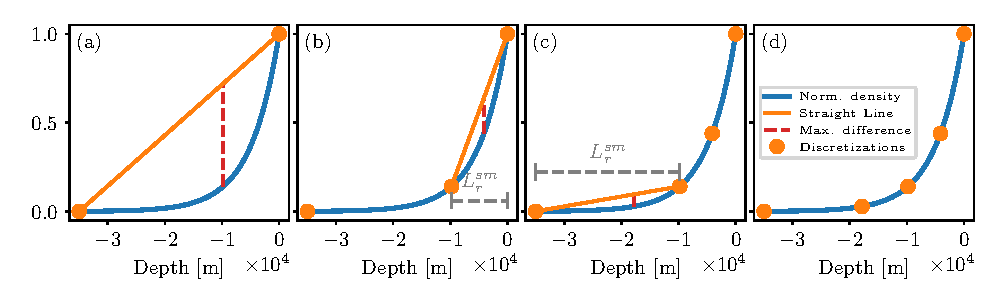
\includegraphics[width=\linewidth]
    {figures/density-based-discretization-algorithm.pdf}
\caption{
    Example application of the density-based discretization algorithm to a non-linear
    density function.
    (a) the normalised density function $\rho_n(r')$ (blue), current boundaries of the
    tesseroid (orange dots), and the linear density function $\rho_l(r')$ (orange line).
    The dashed red line represents the maximum density difference $\Delta \rho (r')$ at
    which the tesseroid would be divided (assuming that the inequality
    \ref{eq:delta-density} is not satisfied).
    (b) second iteration of the algorithm with a new linear density function and maximum
    density difference. The tesseroid would be divided at the depth indicated by the
    dashed red line.
    (c) third iteration of the algorithm.
    (d) final output of the density-based discretization, assuming that all four new
    tesseroids satisfy inequality \ref{eq:delta-density}.
}
\label{fig:density-discretization-algorithm}
\end{figure*}

Once all smaller tesseroids satisfy Eq. \ref{eq:delta-density},
each one is subjected to the adaptive
discretization algorithm described earlier to calculate their gravitational effects.

On the first iteration, the ratio $L_r/L_r^\text{orig} = 1$ because the tesseroid being
divided is the original one.
For future iterations, the ratio will be progressively smaller than one as the
tesseroids get smaller.
This is intended to limit the number of divisions to the ones that will
significantly reduce the numerical error:
dividing a large tesseroid with a small $\text{max}\{ \Delta \rho(r') \}$ would
improve the integration accuracy more than dividing a small tesseroid with a
higher $\text{max}\{ \Delta \rho(r') \}$.
We also do not divide tesseroids with $L_r < 1\ mm$ because any integration errors would
be negligible due to the small mass of the tesseroid..

The higher $\delta$ is, the fewer divisions will be made, and vice-versa.
Thus, it controls how many times the tesseroids will be divided based on the density
function and, indirectly, determines the accuracy and computation time of
numerical integration.
This raises the need to determine a maximum value of $\delta$ that
ensures an acceptable accuracy while minimising the computation time.


\subsection{Software implementation}

We have implemented the algorithms described in the previous sections in the Python
programming language.
The software is based on the pre-existing code for the homogeneous density tesseroid
\citep{Uieda2016}, more specifically the implementation in the Python library Fatiando a
Terra v0.5 \citep{Uieda2013}.
The more time consuming parts of the algorithm are written in the Cython language to
achieve higher performance.
This new code is freely available under the BSD 3-clause open-source license.
It can be downloaded from the online repository
\href{https://github.com/pinga-lab/tesseroid-variable-density}{github.com/pinga-lab/tesseroid-variable-density}.



%%%%%%%%%%%%%%%%%%%%%%%%%%%%%%%%%%%%%%%%%%%%%%%%%%%%%%%%%%%%%%%%%%%%%%%%%%%%%

\section{Determination of the distance-size and delta ratios}

The distance-size ration $D$ of the adaptive discretization and the delta ratio $\delta$
of the density-based discretization determine how many times each tesseroid will be
divided and thus indirectly control the numerical error of the integration.
Optimal values for $D$ and $\delta$ must be determined in order to ensure both
acceptable numerical accuracy and computation efficiency for the algorithm.

\citet{Uieda2016} compared the numerical integration of homogeneous density tesseroids
with the analytical solution of a spherical shell \citep{Mikuska2006,Grombein2013} in
order to obtain default values for the distance-size ratio $D$.
We will follow this idea but for our needs the spherical shell must
have the same density function of radius as our tesseroid model.
Analytical solutions for a variable density spherical shell are not present in the
literature and so they must be obtained first.
We derive the expressions for the gravitational fields of spherical shells with linear
and exponential density functions of radius in Appendix \ref{sec:shell}.

We perform comparisons between the analytical solutions for the spherical shell and the
numerical integration results for linear and exponential density functions.
From these results, we generalize default values for $D$ and $\delta$ that ensure a
numerical error lower than 0.1\% of the spherical shell values.

\begin{table}
\caption{
    Description of the tesseroid models of a spherical shell and computation grids
    used to characterize the accuracy of the numerical integration.
    Every grids consist of a set of $10 \times 10$ points.
}
\label{tab:grids}
\begin{tabular}{lccc}
    Name & Tesseroid size & Grid region (degrees) & Grid height (km)
    \\ \hline
    Pole & $1^\circ \times 1^\circ$ & $0\text{E}/1\text{E}/89\text{N}/90\text{N}$ & 2 \\
    Equator & $1^\circ \times 1^\circ$ & $0\text{E}/1\text{E}/0\text{N}/1\text{N}$ & 2 \\
    Satellite & $1^\circ \times 1^\circ$ & $0\text{E}/1\text{E}/89\text{N}/90\text{N}$ & 260 \\
    Big Grid & $30^\circ \times 30^\circ$ & $0\text{E}/30\text{E}/60\text{N}/90\text{N}$ & 2 \\
\end{tabular}
\end{table}


\subsection{Linear Density}

A spherical shell with a linear density function given by

\begin{equation}
    \rho(r') = ar' + b,
    \label{eq:density-linear}
\end{equation}

\noindent
has an analytical solution given by Eq. \ref{eq:shell-pot-linear}.

The absolute density difference defined on equation
\ref{eq:density-abs-diff} will always be zero for the linear density case.
As a result, the inequality \ref{eq:delta-density} will always be satisfied and no
divisions will ever be performed.
Therefore, the distance-size ratio $D$ of the adaptive discretization algorithm is the
only mechanism that controls the accuracy of the numerical integration.
For this reason, we will only determine the minimum value of $D$ needed in order to
guarantee an acceptable accuracy while ignoring the value of $\delta$.

In order to compare the numerical results with the analytical solution we
must build a spherical shell made of tesseroids.
We use a combination of tesseroid models with different resolutions and compute their
effects on $10 \times 10$ point grids at different heights and locations.
All combinations of models and grids are shown in Table \ref{tab:grids}.
The tesseroid model is composed of a single radial layer.
The combinations in Table \ref{tab:grids} are repeated for two shells with thickness 1
km and 35 km.
The outer radius of both shells are equal to the mean Earth radius and
the density varies linearly (Eq. \ref{eq:density-linear})
with angular coefficient

\begin{equation}
    a = -\frac{3300\text{kg/m$^3$} - 2670\text{kg/m$^3$}}{R - R_1},
\end{equation}

\noindent and linear coefficient

\begin{equation}
    c = \frac{3300\text{kg/m$^3$} -
        2670\text{kg/m$^3$}}{R - R_1} R +
        2670\text{kg/m$^3$},
\end{equation}

\noindent
in which $R$ = 6378.137 km is the mean Earth radius and $R_1$ is the inner radius of the
shell (determined by the thickness).

We compute the gravitational potential ($V$), the vertical component of the gradient
($g_z$), and the diagonal components of the Marussi tensor ($g_{xx}$, $g_{yy}$,
$g_{zz}$) for each of the four tesseroid models and grids in Table
\ref{tab:grids}.
Other components are equal to zero outside of the shell and are thus omitted from the
analysis.
The computations are repeated for values of $D$ ranging from 0.5 to 10 with a step of
0.5.
We then will calculate the maximum absolute difference between these results and the
analytical solutions derived in Appendix \ref{sec:shell}.
The differences are shown in Fig. \ref{fig:D-linear} as relative to the spherical shell
values.
We omit the differences for $g_{xx}$ and $g_{yy}$ because they are equivalent to the
ones obtained for $g_{zz}$.
Finally, we set the optimal value of $D$ as the minimum value at which the corresponding
error of the numerical approximation is lower than 0.1\%.

We observe from Fig. \ref{fig:D-linear} that the relative errors for the
potential and the $g_z$ component fall below the 0.1\% threshold at
$D=1$ and $D=2$, respectively, for both shell thicknesses.
On the other hand, $g_{zz}$ displays a noticeable
difference between the thin and the thick shell: the first one needs a
value of $D$ equal to 8 while the later only a $D$ of 3.

\begin{figure*}
\centering
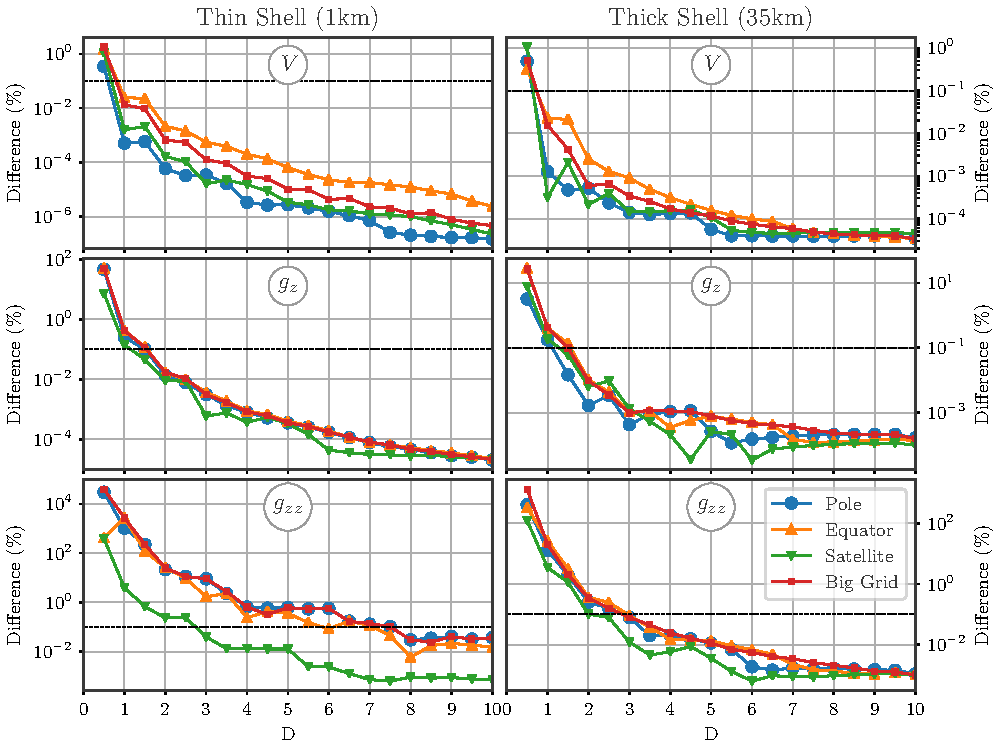
\includegraphics[width=\linewidth]{figures/linear-D.pdf}
\caption{
    Differences between the gravitational fields generated by the tesseroid model
    and the analytical solution for a thin (left) and a thick (right) spherical shell.
    Both models have a linear density function of radius (Eq. \ref{eq:density-linear}).
    The computations were performed on the four combinations described in
    Table \ref{tab:grids}.
    Due to the linearity of the density function, the density-based discretization
    algorithm is not applied.
    Differences are reported as a percentage of the shell values.
    The horizontal dashed black line represents a target difference of 0.1\%.
}
\label{fig:D-linear}
\end{figure*}


\subsection{Exponential Density}

For an exponential density function, the density-based discretization will be applied
before the adaptive discretization algorithm.
This means that optimal values for both the distance-size ratio $D$ and the delta ratio
$\delta$ must be determined.
We perform an error analysis similar to what was done for the linear density case.
However, we only consider the ``Big Grid'' scenario from Table \ref{tab:grids} for the
sake of brevity.

The spherical shell and tesseroid model will have an exponential density function given
by

\begin{equation}
    \rho(r') = A e^{-(r' - R)/b} + C,
\label{eq:density-exp}
\end{equation}

\noindent where

\begin{equation}
    A =
    (3300 \text{kg/m}^3 - 2670 \text{kg/m}^3)
    \left( e^{( R - R_1 )/b} - 1 \right)^{-1},
\end{equation}

\begin{equation}
    C =
    2670 \text{kg/m}^3 - A,
\end{equation}

\noindent $R$ is the mean Earth radius, $R_1$ is the inner radius of the
shell (determined by the thickness), and $b$ is a constant that determines the
variability of the function: a low value of $b$ increases the maximum slope of the
density function.


\subsubsection{$D$-$\delta$ space exploration}

We aim to find a combination of the $D$ and $\delta$ that produces a numerical error
lower than the 0.1\% threshold while minimizing computation time.
We use a grid search method and compute the numerical error for every ($D$, $\delta$)
pair belonging to a grid on the $D$-$\delta$ space (Fig. \ref{fig:grid-search}).
Because this is a time consuming computation, we limit the analysis to a shell of 35 km
thickness and $b = 1\ \text{km}$ (Eq. \ref{eq:density-exp}), which yields a
sharp density variation within the shell.
For optimum algorithm performance, we search for the smallest possible value of $D$ and
the highest possible value of $\delta$.

We compute the relative difference between the numerical and analytical results for the
gravitational potential ($V$), the vertical component of its gradient ($g_z$), and the
$g_{zz}$ component of the Marussi tensor.
The results are shown in Fig. \ref{fig:grid-search}, in which points inside the dotted
lines are the ones that present a numerical error lower than the 0.1\% threshold.
Also shown in Fig. \ref{fig:grid-search} are the $D$ values determined for the linear
density function in the previous section ($D_\text{linear}$).
The values of $D_\text{linear}$ are within the 0.1\% threshold and are the optimum
values of $D$ for $V$ and $g_z$.
The results for $g_{zz}$ are in agreement with those obtained for the linear density
function in the case of a thick shell (Fig. \ref{fig:D-linear}).
Thus, we also choose the conservative value of $D=8$ as the optimum value for $g_{zz}$.
These results indicate that the values of $D_\text{linear}$ can be safely extrapolated
to the exponential case.


\begin{figure}
\centering
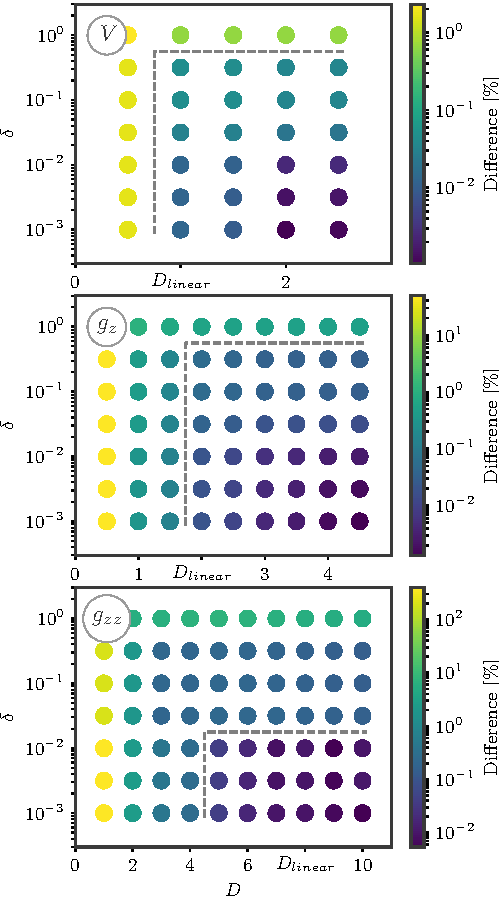
\includegraphics[width=\linewidth]
    {figures/grid-search.pdf}
\caption{
    Numerical error exploration in the $D$-$\delta$ space.
    The percentage difference values were obtained from the comparison
    between the analytical solution and the numerical approximation of
    the gravitational fields ($V$, $g_z$ and $g_{zz}$) generated by a
    spherical shell with an exponential density function (Eq. \ref{eq:density-exp}).
    These comparisons were carried out on the ``Big Grid'' configuration (Table
    \ref{tab:grids}), with a spherical shell of
    35km of thickness, and density function with $b$ of 1km.
    The points inside the dashed line are the ones that present an
    error lower than 0.1\%.
    }
\label{fig:grid-search}
\end{figure}


\subsubsection{Delta ratio determination}

Having chosen values of $D$ equal to linear density case, we are free to explore the
integration error as a function of $\delta$ in more detail and how it varies for
different values of $b$ (Eq. \ref{eq:density-exp}).
We perform the error calculations for the ``Big Grid'' configuration (Table
\ref{tab:grids}) for two spherical shell models with 1km and 35km thickness.
The calculations are repeated for different values of $b$ to examine the error variation
with the sharpness of the density function.
Because larger $\delta$ values result in fewer tesseroid divisions,
our intention is to find the highest value of $\delta$ whose numerical error is bellow
the $0.1\%$ threshold.

Fig. \ref{fig:delta-exponential} shows the density functions and the resulting relative
differences ($V$, $g_z$, and $g_{zz}$) for different values of $b$ and thickness of the
shell and tesseroid model.
The relative difference for $V$ and $g_z$ falls below the 0.1\% threshold for
$\delta = 0.2$ in both the thick and thin shell cases.
On the other hand, optimal values of $\delta$ for $g_{zz}$
are $\delta = 0.2$ for the thin shell and $\delta = 0.01$ for the thick shell.
Once again, we opt for the conservative value of $\delta = 0.01$ and sacrifice
performance for the sake of accuracy.

\begin{figure*}
\centering
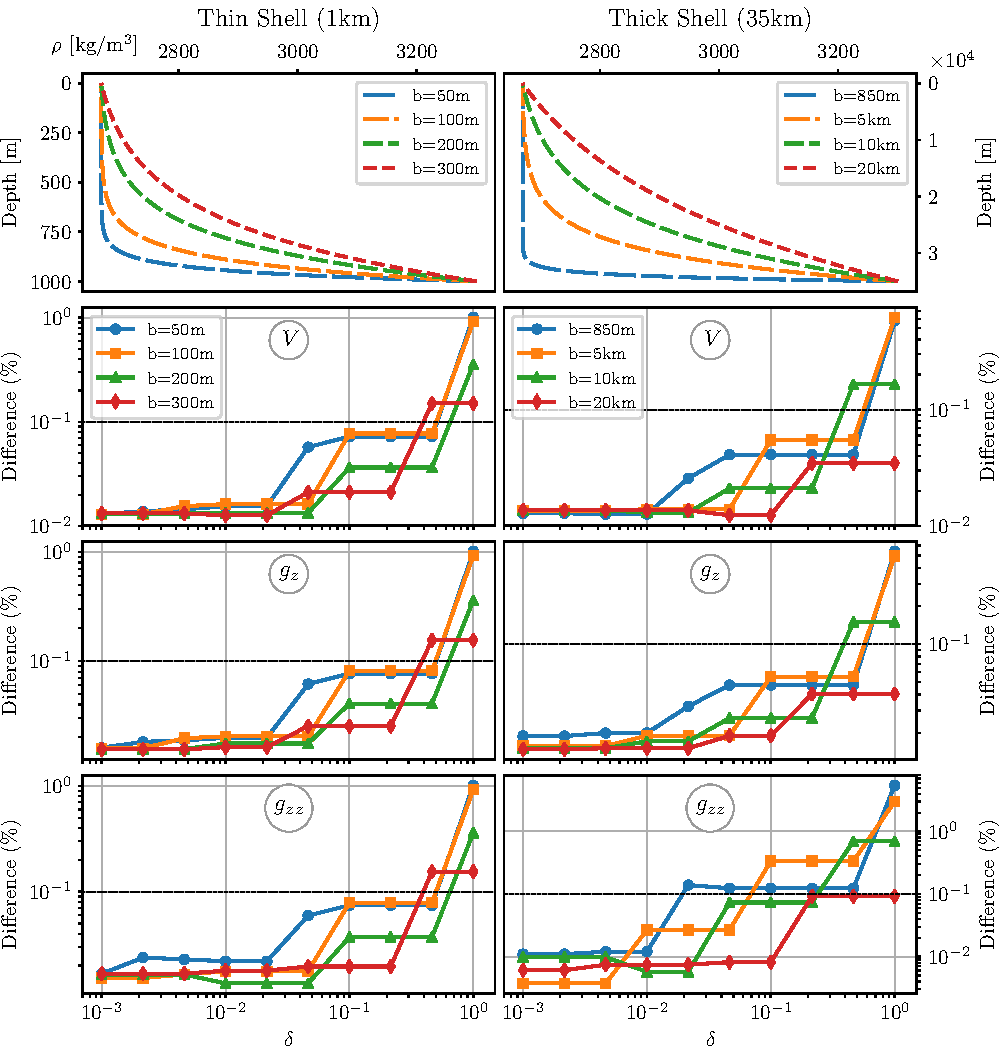
\includegraphics[width=\linewidth]{figures/exponential-delta.pdf}
\caption{
    Numerical error for different exponential density functions and values of the delta
    ratio.
    The top panels show the exponential density functions for different values of $b$
    (Eq. \ref{eq:density-exp}).
    The error computations were performed on the ``Big Grid'' configuration described in
    Table \ref{tab:grids}, with fixed values of the distance-size ratio
    $D$ obtained for the linear density case ($D=1, 2, 8$ for the
    potential, gradient components, and tensor components, respectively).
    The difference is reported as a percentage of the shell values.
    }
\label{fig:delta-exponential}
\end{figure*}


%%%%%%%%%%%%%%%%%%%%%%%%%%%%%%%%%%%%%%%%%%%%%%%%%%%%%%%%%%%%%%%%%%%%%%%%%%%%%%%

\section{Application to the Neuqu\'en Basin}

We applied the new algorithms and optimal values of $D$ and $\delta$ determined
previously to calculate the gravitational effects of the Neuqu\'en Basin:
a sedimentary basin
located to the east of the Andes, between 32$^\circ$S and 40$^\circ$S latitude
(Fig. \ref{fig:neuquen-basin}a).
The basin includes continental and marine siliciclastics, carbonates, and evaporites
accumulated over the Jurassic and the Cretaceous constituting a stratigraphic record up
to 5000m of depth \citep{Howell2005}.

\begin{figure*}
\centering
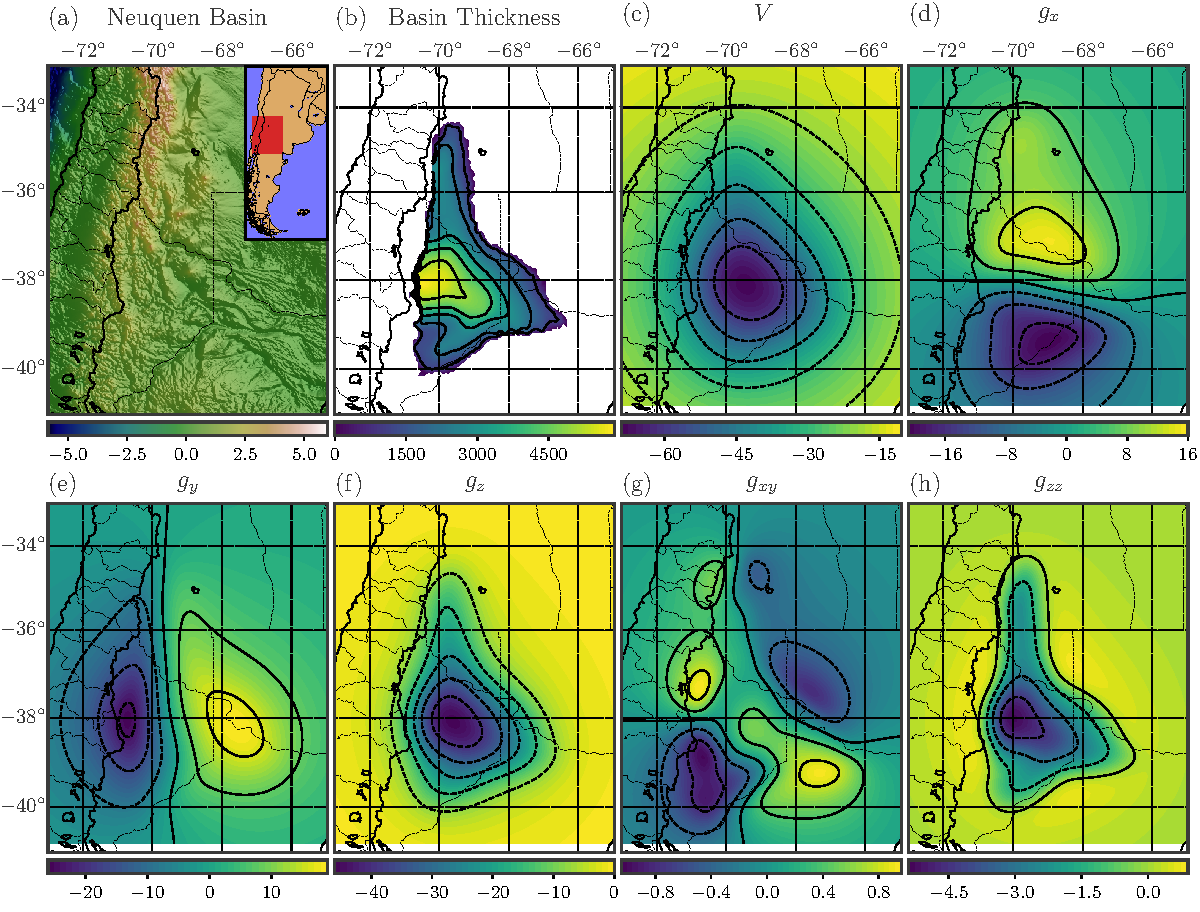
\includegraphics[width=\linewidth]{figures/neuquen-basin.pdf}
\caption{
    Gravitational effects of the Nequ\'en sedimentary basin modelled
    using tesseroids with an exponential density function of depth.
    (a) Topography of the Neuqu\'en Basin (in km) and its location in South America,
    (b) thickness of the sedimentary basin \citep[in meters;][]{Heine2007},
    (c) the exponential density function used to model the basin
        (depth in km and density in kg/m$^3$),
    (d)-(l) computed gravitational fields: potential $V$ (in J/kg), gradient
    components $g_x$, $g_y$ and $g_z$ (in mGal), and Marussi tensor components
    (in Eötvös), calculated at 50km of height over the ellipsoid.
}
\label{fig:neuquen-basin}
\end{figure*}

The thickness of the sediment pack was digitized from \citet{Heine2007} on a regular
grid with a resolution of 0.05$^\circ$ on both longitude and latitude directions
(Fig. \ref{fig:neuquen-basin}b).
We created a tesseroid model of the sediment pack by placing a
$0.05^\circ \times 0.05^\circ$ tesseroid on each node of the grid.
The top of each tesseroid was fixed at 0 m depth and the bottom at corresponding
thickness of the basin.

We must also define a density function for the tesseroid model.
\citet{Sigismondi2012} measured a minimum and maximum density contrast for
the Neuqu\'en basin of -412kg/m$^3$ and -275kg/m$^3$, respectively.
We have chosen an exponential density variation (Eq. \ref{eq:density-exp}) that assumes
the minimum value on the top surface and the maximum at 5858m depth (the thickest part
of the basin), with a value of $b$ equal to 2km.
This density function can be seen on Fig. \ref{fig:neuquen-basin}c.

Finally, we computed the gravitational potential $V$, gradient components $g_x$,
$g_y$ and $g_z$, and the Marussi tensor components $g_{xx}$, $g_{xy}$,
$g_{xz}$, $g_{yy}$, and $g_{zz}$ on a computation grid of $159\times163$ nodes
($0.05^\circ$ spacing on both longitude and latitude) at a 50km height over the
reference ellipsoid.
The resulting fields can be seen in Fig.
\ref{fig:neuquen-basin}d-l.
We have excluded the other components of the Marussi tensor from the Fig.
\ref{fig:neuquen-basin},
although they can be found in the online repository.


%%%%%%%%%%%%%%%%%%%%%%%%%%%%%%%%%%%%%%%%%%%%%%%%%%%%%%%%%%%%%%%%%%%%%%%%%%%%%%%

\section{Conclusions}

We have developed a new methodology to compute the gravitational fields
generated by a tesseroid with a density given by a continuous function of depth.
It numerically solves the integrals that define the gravitational potential,
its gradient, and the Marussi tensor components through the Gauss-Legendre
Quadrature (GLQ).
The accuracy of the numerical integration is automatically controlled by an adaptive
discretization algorithm and a new density-based discretization algorithm.
The former divides the tesseroid in half if the ratio of the distance to the computation
point and the size of the tesseroid is lower than a predefined distance-size ratio $D$.
This algorithm minimises the integration error when the computation point is close to
the tesseroid.
Nevertheless, the adaptive discretization alone is not sufficient to guarantee the
accuracy of the method in case of tesseroids with variable density.

To overcome this challenge, we have developed a density-based discretization algorithm
that divides the tesseroid on the points at which the maximum variations of the density
function takes place.
The density-based discretization is performed before adaptive discretization as a type
of pre-processing step.
The number of divisions performed, and thus the accuracy of the computation, is
controlled by the delta ratio $\delta$.
This new algorithm is intended to minimise the error due to the inability of
the GLQ to produce precise approximations of highly variable density functions.

Because there is no direct relation between the values assigned to $D$ and
$\delta$ with the error of the computation, we had to empirically determine
the minimum value of $D$ and the maximum value of $\delta$ that produce an
acceptable accuracy for each gravitational field, while maintaining an
efficient computation.
The default values of $D$ and $\delta$ must produce accurate computations for
most continuous and smooth densities, that's why we have chosen two density
functions in order to establish them: a linear and an exponential one.

In the linear density case, the densty-based discretization algorithm is not
applied due to how it's build, so only a default value of $D$ had to be
determined.
By comparing the analytical solutions of the gravitational fields generated by
a spherical shell with the ones produced by the numerical model for different
values of $D$, we have obtained default values for the distance-size ratio of
1, 2 and 8 for the potential, its gradient and the Marussi tensor components,
respectively.
From these comparisons we can guarantee a precision of 0.1\% or greater on the
computations of the gravitational fields generated by any tesseroid with a
linear density.

The exponential density case is more complex, due to the fact that both $D$
and $\delta$ must be determined simultaneously.
We have explored regular gridded points in the $D$, $\delta$ space and
computed the percentage difference between the analytical solutions for a
spherical shell and the numerical model.
We had to take into account that the $D$ values cannot be lower than the ones
determined for the linear density case due to the fact that they must
guarantee acceptable accuracy for every continuous density function, including
the linear one.
From these comparisons we have concluded that the more efficient computations
take places when the $D$ values obtained in the linear density scenario are
used, i.e. the minimum ones.
This can be understood in terms of which kind of discretization produces more
subdivisions: a higher $D$ may produce more discretizations than a lower
$\delta$ because the first one divides the tesseroid in the radial, longitude
and latitude directions, while the latter only divides it in the radial
direction.
In conclusion, we found out that keeping the $D$ values as the ones obtained
for the linear density case, a $\delta = 0.2$ is needed for the computation of
the potential and its gradient components, while a $\delta = 0.01$ must be
used for the Marussi tensor components in order to ensure a 0.1\% precision.

In order to implement this new methodology we have developed a Python code
that carries out both discretization algorithms and the gravitational field
computation through the GLQ. It's freely available under the BSD 3-clause
open-source license and can be downloaded from
\todo[inline]{add repo url}

Finally, we have shown how this new method performs under a real data example:
we have computed the gravitational fields generated by the Neuqu\'en
sedimentary basin through a tesseroid model with an increasing exponential
density in depth on a regular grid at a computation height of 50km over the
reference ellipsoid.


%%%%%%%%%%%%%%%%%%%%%%%%%%%%%%%%%%%%%%%%%%%%%%%%%%%%%%%%%%%%%%%%%%%%%%%%%%%%%%%

\section{Acknowledgments}

We are indebted to the developers and maintainers of the open-source
software without which this work would not have been possible.

%%%%%%%%%%%%%%%%%%%%%%%%%%%%%%%%%%%%%%%%%%%%%%%%%%%%%%%%%%%%%%%%%%%%%%%%%%%%%%%

\bibliographystyle{gji}
\bibliography{references}

\appendix

\section{Analytical Solutions for Spherical Shell}
\label{sec:shell}

\begin{figure}
\centering
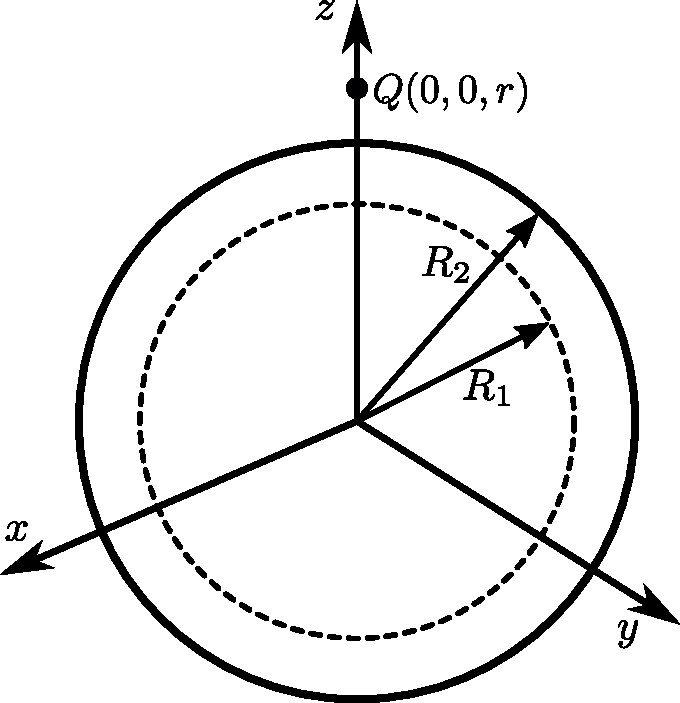
\includegraphics[width=0.7\linewidth]{figures/spherical-shell.pdf}
\caption{
    Spherical shell with inner and outer radii $R_1$ and $R_2$, respectively.
    The computation point $Q$ is located on the $z$ axis at a distance $r$ from
    the origin of the coordinates system.
    For our purposes we will assume that $Q$ is outside of the shell,
    i.e. $r > R_2$.
}
\label{fig:spherical-shell}
\end{figure}

Consider a spherical shell with inner radius $R_1$ and outer radius $R_2$,
whose density is a function $\rho(r')$ of the radial coordinate
(Fig. \ref{fig:spherical-shell}).
The gravitational potential generated by the shell on an arbitrary external
point $Q$ can be written as follows:

\begin{equation}
    V_\text{sh}(\phi, \lambda, r) = G
    \int\limits_0^{2\pi}
    \int\limits_{-\frac{\pi}{2}}^\frac{\pi}{2}
    \int\limits_{R_1}^{R_2}
    \frac{\rho(r')}{\ell} {r'}^2 \cos\phi' \,
    dr' d\phi' d\lambda',
\end{equation}

\noindent where $\ell$ is defined in equation \ref{eq:ell}.

For $Q$ located along the $z$ axis (i.e., $\phi=90^\circ$) at a distance $r$ from the
origin, equation \ref{eq:ell} simplifies to:

\begin{equation}
    \ell = \sqrt{r'^2 + r^2 - 2 r r' \sin\phi'}.
\end{equation}

\noindent
Because of the rotational symmetry along the $z$ axe, the integration in $\lambda'$ is
straightforward:

\begin{equation}
    V_\text{sh}(r) = 2\pi G
    \int\limits_{-\frac{\pi}{2}}^\frac{\pi}{2}
    \int\limits_{R_1}^{R_2}
    \frac{\rho(r') {r'}^2 \cos\phi'}{\sqrt{r'^2 + r^2 - 2 r r' \sin\phi'}}
    \, dr' d\phi',
\end{equation}

\noindent
while the integration in $\phi'$ can be performed independently of the density function.
Making use of SymPy \citep{sympy2017}, a Python library for symbolic mathematics, we
obtained the following expression for the potential:

\iftwocol{
\begin{equation}
    \begin{split}
        V_\text{sh}(r) = 2\pi G
        \int\limits_{R_1}^{R_2}
        \Big[ & \sqrt{r^2 + r'^2 + 2rr'} - \\
        & \sqrt{r^2 + r'^2 - 2rr'}
        \Big] \frac{r'\rho(r')}{r} \, dr'.
    \end{split}
\label{eq:shell-pot-sqrts}
\end{equation}
}{
\begin{equation}
    V_\text{sh}(r) = 2\pi G
    \int\limits_{R_1}^{R_2}
    \Big[ \sqrt{r^2 + r'^2 + 2rr'}  -
    \sqrt{r^2 + r'^2 - 2rr'}
    \Big] \frac{r'\rho(r')}{r} \, dr'.
\label{eq:shell-pot-sqrts}
\end{equation}
}

Because the computation point $Q$ is outside of the shell, $r > r'$ and the square roots
in equation \ref{eq:shell-pot-sqrts} simplify to

\begin{equation}
    \sqrt{r^2 + r'^2 + 2rr'} = |r + r'| = r + r',
\end{equation}

\begin{equation}
    \sqrt{r^2 + r'^2 - 2rr'} = |r - r'| = r - r',
\end{equation}

\noindent which leads to the following expression for the potential:

\begin{equation}
    V_\text{sh}(r) = \frac{4\pi G}{r}
    \int\limits_{R_1}^{R_2} {r'}^2 \rho(r') \, dr'.
\label{eq:shell-pot}
\end{equation}

The gradient and the Marussi tensor of potentials that
depends solely on $r$ have only a few non zero components: the vertical
component of the gradient ($g_z$) and the diagonal components of the
tensor ($g_{xx}$, $g_{yy}$, $g_{zz}$).
Following \citet{Grombein2013}:

\begin{equation}
    g_z(r) = \frac{V_\text{sh}(r)}{r},
\end{equation}

\begin{equation}
    g_{xx}(r) = g_{yy}(r) = -\frac{V_\text{sh}(r)}{r^2}
\end{equation}

\begin{equation}
    g_{zz}(r) = \frac{2V_\text{sh}(r)}{r^2}.
\end{equation}

From Eq. \ref{eq:shell-pot} we can obtain expressions for gravitational potential for
different density functions.
For a linear density function

\begin{equation}
    \rho(r') = ar' + b\ ,
\end{equation}

\noindent
the gravitational potential at any external point is

\begin{equation}
    V_\text{sh}^\text{lin}(r) = \pi G \left[
    a \frac{R_2^4 - R_1^4}{r} +
    b \,\frac{4}{3} \frac{R_2^3 - R_1^3}{r} \right].
    \label{eq:shell-pot-linear}
\end{equation}

\noindent The first term on this equation reproduces the potential generated
by a spherical shell with variable density $\rho(r') = ar'$, while the second
term constitutes the potential generated by a spherical shell with homogeneous
density $\rho = b$ \citep{Mikuska2006,Grombein2013}.

An exponential density function that assumes the values of $\rho_\text{out}$ and
$\rho_\text{in}$ on the shell's outer and inner surfaces, respectively, can be defined
as follows:

\begin{equation}
    \rho(r') = A e^{-(r' - R)/b} + C,
\end{equation}

\noindent where

\begin{equation}
    A = (\rho_\text{in} - \rho_\text{out})
        \left( e^{( R_2 - R_1 )/b} - 1 \right)^{-1},
\end{equation}

\begin{equation}
    C = \rho_\text{out} - A,
\end{equation}

\noindent $R$ is the mean Earth radius, and $b$ is a constant
that determines the variability of the function: a low value of $b$
increases the maximum slope of the density function.

The analytical solution of the gravitational potential generated by a
spherical shell with a density function is

\iftwocol{
\begin{equation}
    \begin{split}
        V_\text{sh}^\text{exp}(r) = \frac{4\pi G}{r}
        Ab
        \Big[
        & (R_1^2 + 2R_1 b + 2b^2)e^{-\frac{R_1 - R}{b}} - \\
        & (R_2^2 + 2R_2 b + 2b^2)e^{-\frac{R_2 - R}{b}}
        \Big] + \\
        & \frac{4 \pi G}{3 r} C (R_2^3 - R_1^3).
    \end{split}
\label{eq:shell-pot-exp}
\end{equation}
}{
\begin{equation}
    V_\text{sh}^\text{exp}(r) = \frac{4\pi G}{r}
    Ab \, e^\frac{R}{b}
    \Big[
    (R_1^2 + 2R_1 b + 2b^2)e^{-\frac{R_1}{b}} -
    (R_2^2 + 2R_2 b + 2b^2)e^{-\frac{R_2}{b}}
    \Big] +
    \frac{4 \pi G}{3 r} C (R_2^3 - R_1^3).
\label{eq:shell-pot-exp}
\end{equation}
}


\end{document}

